% !TEX TS-program = pdfLaTeX+shellescape
% !TEX encoding = UTF-8 Unicode

\documentclass[class=beamer,tikz]{standalone}
\setbeamertemplate{navigation symbols}{} % For delete the navigation symbols
\usefonttheme{professionalfonts}
\usepackage{luatexja}
% \usepackage{pgfplots}
% \pgfplotsset{compat=1.17}

\usepackage{colortbl,array,xcolor}
\usepackage{amsmath,amsfonts}

\begin{document}
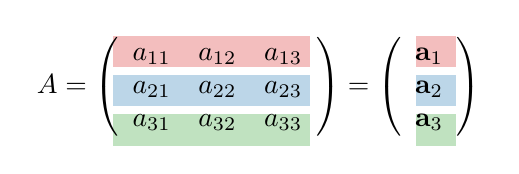
\begin{tikzpicture}
    \definecolor{tab_red}{HTML}{d62728}
    \definecolor{tab_blue}{HTML}{1f77b4}
    \definecolor{tab_green}{HTML}{2ca02c}
    % \draw[help lines] (0,0) grid (8,5);
    \path[fill=tab_red!30] (1.65,4.25) rectangle (4.15,4.65);
    \path[fill=tab_blue!30] (1.65,3.75) rectangle (4.15,4.15);
    \path[fill=tab_green!30] (1.65,3.25) rectangle (4.15,3.65);
    \path[fill=tab_red!30] (5.5,4.25) rectangle (6.0,4.65);
    \path[fill=tab_blue!30] (5.5,3.75) rectangle (6.0,4.15);
    \path[fill=tab_green!30] (5.5,3.25) rectangle (6.0,3.65);

    \node (matrix) at (3.5,4) {
        $A = \left(\begin{array}{ccc}
            a_{11} & a_{12} & a_{13} \cr 
            a_{21} & a_{22} & a_{23} \cr 
            a_{31} & a_{32} & a_{33}
        \end{array}\right) = \left(\begin{array}{ccc}
            \mathbf{a}_1 \cr 
            \mathbf{a}_2 \cr 
            \mathbf{a}_3
        \end{array}\right)$
    };
\end{tikzpicture}
\end{document}